\subsection{When}\label{when}
\begin{center}

\textit{Quali sono le ultime novità? Quando è stato aggiornato l'ultima volta?}

\end{center}
\begin{flushleft}
Il sito non presenta in modo agevole tali contenuti nella homepage, questi possono
essere raggiunti solamente scrollando fino all'ultima pagina (di scroll) presente
nella homepage. Alternativamente è possibile selezionare la sezione (Blog) presente
nel menù di navigazione.
    \begin{figure}[ht]
    \centering
    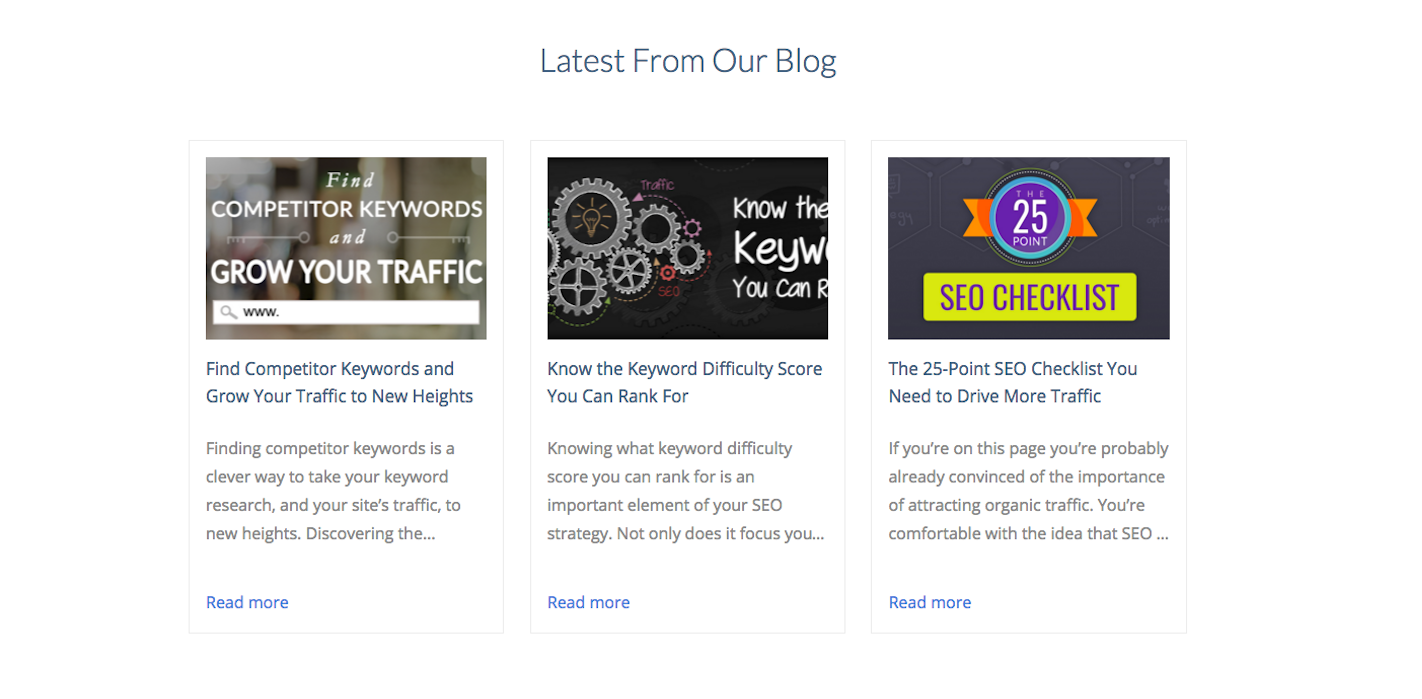
\includegraphics[scale=0.30,keepaspectratio]{{figure/3/when0}.png}
    \caption{Presentazione dell'asse when}
    \end{figure}
    \FloatBarrier 
Questo tipo di asse informativo non viene presentato in modo immediato e
chiaro, infatti (come si può notare dalla figura) gli articoli non riportano
la data in cui sono stati scritti e quindi non permettono all'utente di capire che 
frequenza di aggionarmento ha il sito. \\
Risultato : \textbf{5}
\end{flushleft}